\section{Properties of Wigner distributions}
\label{app:wigner}

Here we present important properties of the phase-point operators and the Wigner distribution that are used throughout the paper.

\begin{proposition}\label{thm:aproperties}
    For any dimension $d$, the phase-point operators satisfy:
    \begin{enumerate}
        \item[(i)]\label{en:a1} Hermiticity and unitarity: $A_{\bmx}^\dagger = A_{\bmx} = A_{\bmx}^{-1}$;
	    \item[(ii)]\label{en:a2} Closure under transposition: $A_{(x, p)}^T = A_{(x, p)}$;
	    \item[(iii)]\label{en:a3} Unit trace for odd $d$: $\tr[A_{\bmx}] = 1$;
	    \item[(iv)]\label{en:a4} Completeness relation: $\sum_{\bmz \in \cal{P}_d} A_{\bmz} = d\id$;
	    \item[(i)]\label{en:a5} Orthogonality: $\tr[A_{\bmx}^\dagger A_{\bm{x'}}] = d \delta_{\bmx,\bm{x'}}$.
	\end{enumerate}
\end{proposition}
\begin{proof}
	All properties follow from the definition in~\cref{eq:ax} along with properties of the displacement operator $D_{\bmx}$ and can be found in the literature, e.g.~\cite{cit:veitch,Vourdas_2004,cit:gross3}
\end{proof}

\begin{proposition}\label{thm:wstate}
  The Wigner distribution of a state $\rho \in \cal{B}(\cal{H}_d)$ is
  \begin{enumerate}
    \item[(i)]\label{en:w1} Real valued: $\W{\rho} \in \mathbb{R}^{d^2}$;
    \item[(ii)]\label{en:w2} Normalised: $\sum_{\bmz \in \cal{P}_d} \W[\bmz]{\rho}=1$;
    \item[(iii)]\label{en:w3} Bounded: $\abs{\W[\bmx]{\rho}} \leq \frac{1}{d}$.
    \item[(iv)]\label{en:w4} Additive under mixing: \vspace{2pt}\\
    $\W[\bmx]{p\rho_1 + (1-p)\rho_2} = p\W[\bmx]{\rho_1} + (1-p)\W[\bmx]{\rho_2}$;
    \item[(v)]\label{en:w5} Multiplicative under tensor products: \vspace{2pt}\\
    $\W[\bmx_A \oplus \bmx_B]{\rho_A \otimes \rho_B} = \W[\bmx_A]{\rho_A}\W[\bmx_B]{\rho_B}$.
	\end{enumerate}
\end{proposition}
\begin{proof}
	Proof of all properties can be found in the literature~\cite{cit:veitch,Vourdas_2004,cit:gross3,Wang_2019} except for property (iii) which we prove here.
	
Let $\{\lambda_i\}_{i \in \mathbb{Z}_d}$ be the (non-negative) eigenvalues of $\rho$, summing to 1.
Let $\{\alpha_{\bmx,i}\}_{i \in \mathbb{Z}_d}$ be the eigenvalues of $A_{\bmx}$. For any $\bmx, \alpha_{\bmx,i} \in \{-1, 1\}$, due to the hermiticity and unitarity of the phase-point operators. 
Then,
\begin{align}
	\abs{\W{\rho}{\bmx}} &= \frac{1}{d}\abs{\tr[A_{\bmx} \rho]} \leq \frac{1}{d} \abs{\sum_i \alpha_{\bmx,i} \lambda_i} \nonumber\\ &\leq \frac{1}{d}\sum_i \lambda_i = \frac{1}{d}.
\end{align}
The first inequality follows from Theorem 1 of~\cite{cit:mirsky} for the trace of complex matrices, while the second is the Cauchy-Schwarz inequality.
\end{proof}

\begin{proposition}
    \label{thm:wchannel}
    The Wigner distribution of a $\cptp$ operation $\E: \cal{B}(\cal{H}_{d_A}) \mapsto \cal{B}(\cal{H}_{d_B})$ is
    \begin{enumerate}
        \item[(i)]\label{en:wo1} Real-valued: $\W{\E} \in \mathbb{R}^{d^2} \times \mathbb{R}^{d^2}$;
        \item[(ii)]\label{en:wo2} Normalised: $\sum_{\bmz \in \cal{P}_{d_B}} \W[\bmz|\bmx]{\E} = 1$ \\ 
        for any $\bmx \in \cal{P}_{d_A}$;
        \item[(iii)]\label{en:wo3} Bounded: $\abs{\W[\bmy|\bmx]{\E}} \leq \frac{d_A}{d_B}$;
	    \item[(iv)]\label{en:wo4} Transitive: $\W[\bmy]{\E(\rho)} = \sum_{\bmz \in \cal{P}_{d_A}} \W[\bmy|\bmz]{\E} \W[\bmz]{\rho}$ for any $\bmy \in \cal{P}_{d_B}$.
    \end{enumerate}
\end{proposition}
If $d_A = d_B$, and in particular if operation $\E$ maps a Hilbert space onto itself, then the stochasticity condition $\abs{\W[\bmy|\bmx]{\E}} \leq 1$ is satisfied.
\begin{proof}
	Proof of all properties are provided by Wang \textit{et al.}~\cite{Wang_2019} except for property (iii) which is a direct consequence of the definition of $\W{\E}$ and the corresponding property (iii) in~\cref{thm:wstate}.
\end{proof}

%%%%%%%%%%%%%%%%%%%%%%%%%%%%%%%%%%%%%%%%

\section{Properties of majorization}
\label{app:major}

\subsection{Simple--majorization equivalence conditions}

In the unital fragment, namely the limit of infinite temperature, $\beta = 0$, the free state is the maximally mixed state $\frac{1}{d}\id$ with uniform Wigner distribution $\frac{1}{d}\bm{1}  = (\frac{1}{d},\dots,\frac{1}{d})$.
This fragment is governed by simple majorization and we first prove strong equivalences for this type of majorization.
\begin{proposition}\label{prop:major}
Given $\bmx, \bmy \in \mathbb{R}^n$ the following statements are equivalent:
 \begin{enumerate}
	\item[(i)]\label{en:m1} $\bmx \prec \bmy$;
	\item[(ii)]\label{en:m2} $\bmx = B \bmy$ for bistochastic $B$;
	\item[(iii)]\label{en:m3} $\sum\limits_{i=1}^n \abs{x_i - t} \leq \sum\limits_{i=1}^n \abs{y_i - t}$ for all $t \in \mathbb{R}$;
	\item[(iv)]\label{en:m4} $\sum\limits_{i=1}^n (x_i - t)^+ \leq \sum\limits_{i=1}^n (y_i - t)^+$ for all $t \in \mathbb{R}$ and \vspace{5pt}\\ $\sum\limits_{i=1}^n x_i = \sum\limits_{i=1}^n y_i$, where $(x)^+ = \max{\{x, 0\}}$;
	\item[(v)]\label{en:m5} $L_{\bmx}(k) \leq L_{\bmy}(k)$ for $k=1,\dots,n-1$	and \vspace{5pt}\\ $L_{\bmx}(n) = L_{\bmy}(n)$.
 \end{enumerate}
\end{proposition}
\begin{proof}
	These simple majorisation properties are well-known and proofs can be found in~\cite{cit:marshall,cit:bhatia,cit:nielsen,cit:lostaglio}.
	The equivalence between (i) and (ii) is the statement of the Hardy, Littlewood and Polya theorem.
\end{proof}

\subsection{Embedding map}

Any $\bmd$--majorization problem can be rephrased as a simple majorization problem in a higher dimensional space via the embedding map.
\begin{definition}
  The embedding map $\Gamma_{\bmd}:\mathbb{R}^n \mapsto \mathbb{R}^N, N = \sum\limits_{i=1}^n d_i$ is the function
  \begin{equation}
    \Gamma_{\bmd}(\bmw) = \bigoplus_{i=1}^n w_i\  \frac{1}{d_i}\bm{1},
  \end{equation}
where $\bm{1}/d_i$ is the $d_i$--dimensional uniform distribution.
The left inverse $\Gamma_{\bmd}^{-1}: \mathbb{R}^N \mapsto \mathbb{R}^n$ is defined to sum up the elements in each block of $\Gamma_{\bmd}(\bmw)$, so that
  \begin{equation}
     \Gamma_{\bmd}^{-1}(\oplus_{i=1}^n w_i \bm{1}/d_i) = \bmw.
  \end{equation}
  This is not a right inverse, because $\Gamma_{\bmd}$ is not surjective.
\end{definition}
The direct sum simply amounts to listing the uniform distributions one after the other.
The embedding map maps the Gibbs distribution to the uniform distribution, $\Gamma_{\bmd}(\bmd) = \bm{1}/N$.
Then, a non-increasing ordering $\Gamma_{\bmd}(\bmz)^\downarrow$ in the new space, corresponds to the so-called ``$\beta$-ordering'' of the original vector denoted by the permutation $\pi$ in~\cref{def:lc}, mapping $(w_i/d_i) \mapsto (w_i/d_i)^\downarrow$ for all $i=1,\dots,n$.

\subsection{\textit{d}-majorization equivalence conditions}

We take the opportunity here	 to simply list useful equivalent statements for $\bmd$--majorisation.

\begin{proposition}\label{prop:dmajor}
Given $\bmx, \bmy, \bmd \in \mathbb{R}^n$, such that the components of $\bmd$ are positive, the following statements are equivalent:
  \begin{enumerate}
    \item[(i)] $\bmx \prec_{\bmd} \bmy$;
    \item[(ii)] $\Gamma_{\bmd}({\bmx}) \prec \Gamma_{\bmd}({\bmy})$;
    \item[(iii)]\label{en:tm3} $\sum\limits_{i=1}^n \abs{x_i - t d_i} \leq \sum\limits_{i=1}^n \abs{y_i - t d_i}$ for all $t \in \mathbb{R}$;
    \item[(iv)] $\sum\limits_{i=1}^n (x_i - t d_i)^+ \leq \sum\limits_{i=1}^n (y_i - t d_i)^+$ for all $t \in \mathbb{R}$ and \vspace{5pt}\\ $\sum\limits_{i=1}^n x_i = \sum\limits_{i=1}^n y_i$;
    \item[(v)] $L_{\bmx|\bmd}(k) \leq L_{\bmy|\bmd}(k)$ for $k=1,\dots,n-1$	 and \vspace{5pt}\\ $L_{\bmx|\bmd}(n) = L_{\bmy|\bmd}(n)$.
  \end{enumerate}
\end{proposition}
\begin{proof}$ $\vspace{-12pt}\\
\begin{enumerate}
	\item[1$\leftrightarrow2$]
	Suppose there exists a $\bmd$--stochastic $S$ such that $\bmx = S\bmy$ and let $B = \Gamma_{\bmd} \circ S \circ \Gamma_{\bmd}^{-1}$.
$B$ is a $N$--dimensional bistochastic matrix, since composition of stochastic matrices is stochastic and $(\Gamma_{\bmd} \circ S \circ \Gamma_{\bmd}^{-1}) (\frac{1}{N}\bm{1}) = (\Gamma_{\bmd} \circ S) (\bm{d}) = \Gamma_{\bmd}(\bm{d}) = \frac{1}{N}\bm{1}$. Then, $B$ maps $\Gamma_{\bmd}({\bmy})$ to $\Gamma_{\bmd}({\bmx})$.
	Conversely, given $B$, let $S = \Gamma_{\bmd}^{-1} \circ B \circ \Gamma_{\bmd}$.
	Similarly, $S$ is a $\bmd$--stochastic matrix that maps $\bmy$ to $\bmx$.
	\item[$2\leftrightarrow3$]\hspace{-5pt}, $2\leftrightarrow4$, $2\leftrightarrow5$ These three statements are equivalent to statements (iii), (iv), (v) in~\cref{prop:major} respectively, for the embedded vectors $\Gamma_{\bmd}({\bmx}), \Gamma_{\bmd}({\bmy})$, which becomes apparent by rewriting
	\begin{align*}
	&\sum\limits_{i=1}^n \abs{x_i - t d_i} = \sum\limits_{i=1}^n d_i \abs{\frac{x_i}{d_i} - t} = \sum\limits_{i=1}^N \abs{\Gamma_{\bmd}(\bmx)_i - t}, \\
	&\sum\limits_{i=1}^n (x_i - t d_i)^+ = \sum\limits_{i=1}^N (\Gamma_{\bmd}(\bmx)_i - t)^+, \\
	&L_{\bmx|\bmd}(k) = L_{\Gamma_{\bmd}(\bmx)}(k'), \text{with}\ k=1,\dots,n\ \\
	&\text{and}\ k'=1,\dots,N, \nonumber
	\end{align*} 
and similarly for the right hand sides of the inequalities.
\end{enumerate}
\vspace{-19pt}
\end{proof}

%%%%%%%%%%%%%%%%%%%%%%%%%%%%%%%%%%%%%%%%

\section{Technical properties of $\sigma$--fragments}
\label{app:frag}

In this section, we provide some useful technical properties of general $\sigma$--fragments.

\begin{proposition}\label{thm:frag_app}
    Let $\R_\sigma = (\O_\sigma, \F_\sigma)$ be a $\sigma$--fragment of magic theory $\R = (\O, \F)$. 
    The following statements hold:
    \begin{enumerate}
        \item No $\sigma$--fragment is empty.
        \item If a free operation leaves two states invariant, then it also leaves their mixtures invariant, 
        \begin{equation*}
            \O_{\sigma} \cap \O_{\sigma'} \subseteq \O_{p\sigma + (1-p)\sigma'}\ \text{for any}\ p \in [0,1].
        \end{equation*}
    \end{enumerate}
\end{proposition}
\begin{proof}$ $\vspace{-12pt}\\

\begin{enumerate}
    \item The identity channel $1_{\rm{C}}: \D \mapsto \D$ belongs to every $\sigma$--fragment, as $1_{\rm{C}} \in \O$ and $1_{\rm{C}}\sigma = \sigma$ for all $\sigma \in \F$.
    
    \item Let $\E \in \O_{\sigma} \cap \O_{\sigma'}$.
    Then $\E \in \cptp$ and corresponds to stochastic Wigner distribution $\W{\E}$ such that $\W{\E} \W{\sigma} = \W{\sigma}$ and $\W{\E} \W{\sigma'} = \W{\sigma'}$.
    Then, $\W{\E} \W{p\sigma + (1-p)\sigma'} = \W{p\sigma + (1-p)\sigma'}$ for any $p \in [0,1]$ due to the additive property~\ref{en:w4} of the Wigner distribution, implying that state $p\sigma + (1-p)\sigma'$ is also left invariant by $\E$.
\end{enumerate}
\vspace{-20pt}
\end{proof}

Any free state $\sigma \in \F$ corresponds to a $d^2$--dimensional probability distribution $\W{\sigma}$ and any free operation $\E \in \O$ corresponds to a $d^2 \times d^2$ stochastic matrix (or conditional probability distribution) $\W{\E}$.
Note that these mappings are one-to-one due to the orthogonality of the phase-point operators as an operator basis.

Note further that free states $\F$ are mapped onto a \emph{strict subset} of the set of probability distributions.
As a counterexample, the sharp $d^2$--dimensional probability distribution $(1, 0, \dots, 0)$ does not correspond to any qudit Wigner distribution because of the boundedness condition in~\cref{thm:wstate}.

Similarly, not all stochastic matrices correspond to completely positive operations.
As an example, consider the permutation matrix
\begin{equation}
    \Pi_X = \begin{psmallmatrix}
        0 & 1 & 0 & 0 & 0 \\
        0 & 0 & 0 & 0 & 1 \\
        0 & 0 & 0 & 1 & 0 \\
        1 & 0 & 0 & 0 & 0 \\
        0 & 0 & 1 & 0 & 0
    \end{psmallmatrix} \otimes \begin{psmallmatrix}
        0 & 0 & 1 & 0 & 0 \\
        0 & 0 & 0 & 0 & 1 \\
        0 & 0 & 0 & 1 & 0 \\
        1 & 0 & 0 & 0 & 0 \\
        0 & 1 & 0 & 0 & 0    
    \end{psmallmatrix} \in {\rm{S}}_5({\W{\frac{1}{5}\id}}).
\end{equation}
It preserves the uniform distribution $\W{\frac{1}{5}\id}$, but it does not correspond to any positive (hence quantum) operation.

We now prove a result referenced in~\cref{sec:lc}.
\begin{proposition}\label{thm:elbows}
	Let $\rho, \tau$ be two quantum states with Lorenz curves $\lc{\rho}{\sigma}(x), \lc{\tau}{\sigma}(x)$ in the $\sigma$--fragment.
	
	Let $t$ be the number of elbows of $\lc{\tau}{\sigma}(x)$ at locations $x_1, \dots, x_t$.
	
	Then, $\lc{\rho}{\sigma}(x) \geq \lc{\tau}{\sigma}(x)$ for all $x \in [0,1]$ iff $\lc{\rho}{\sigma}(x_{i}) \geq \lc{\tau}{\sigma}(x_{i})$ for all $i =1,\dots,t$.
\end{proposition}
\begin{proof}	
	$\lc{\rho}{\sigma}(x) \geq \lc{\tau}{\sigma}(x)$ for all $x \in [0,1]$ trivially implies $\lc{\rho}{\sigma}(x_{i}) \geq \lc{\tau}{\sigma}(x_{i})$ for all $i = 1,\dots,n'$.
	
	Conversely, assume that $\lc{\rho}{\sigma}(x_{i}) \geq \lc{\tau}{\sigma}(x_{i})$ for all $i = 1,\dots,r$.
	First, let $x_0 = 0$ and $x_{n'+1} = 1$, so that $\lc{\rho}{\sigma}(x_0) = \lc{\tau}{\sigma}(x_0) = 0$ and $\lc{\rho}{\sigma}(x_{n'+1}) = \lc{\tau}{\sigma}(x_{n'+1}) = 1$.
	Hence, we can extend the set of elbows $E$ to $E' = E \cup \{x_0, x_{n'+1}\}$.
	
	Pick two consecutive locations $x_{i}, x_{i+1}$ in $E'$ and consider the line segment $\ell_\tau(x)$ connecting points $(x_{i}, \lc{\tau}{\sigma}(x_{i}))$ and $(x_{i+1}, \lc{\tau}{\sigma}(x_{i+1}))$ as well as the line segment $\ell_\rho(x)$ connecting points $(x_{i}, \lc{\rho}{\sigma}(x_{i}))$ and $(x_{i+1}, \lc{\rho}{\sigma}(x_{i+1}))$.
	This is illustrated in~\cref{fig:elbows_proof}.
\begin{figure}[h]
    \centering
    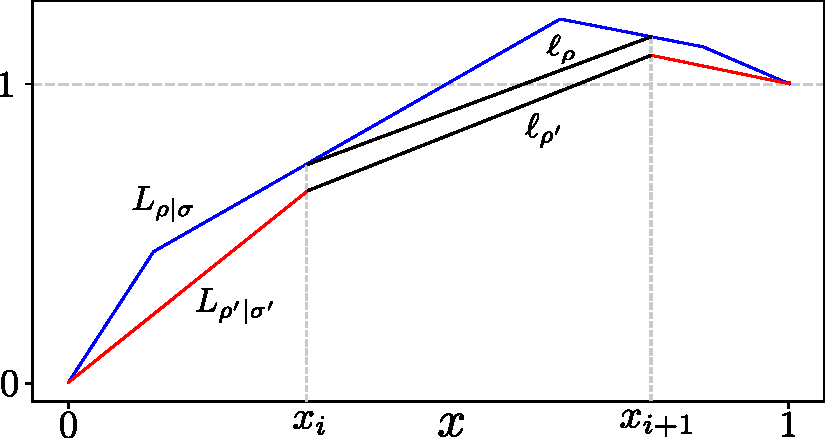
\includegraphics[scale=0.6]{figs/elbows_proof.pdf}
    \caption{\textbf{Illustration of~\cref{thm:elbows}}.
    }
    \label{fig:elbows_proof}
\end{figure}

	Due to concavity of $\lc{\rho}{\sigma}$, it is clear that for all $x \in [x_{i}, x_{i+1}]$, we have $\lc{\rho}{\sigma}(x) \geq \ell_\rho(x) \geq \ell_\tau(x) = \lc{\tau}{\sigma}(x)$.
	This argument can be made in all intervals $[x_{i}, x_{i+1}]$ with $i=0,\dots,n'$, so the proof is complete.
\end{proof}
This theorem is of practical importance in calculating the necessary distillation constraints derived via majorization in $\sigma$--fragments.

%%%%%%%%%%%%%%%%%%%%%%%%%%%%%%%%%%%%%%%%

\section{Lorenz curves in the unital fragment}
\label{app:lcsu_technical}

\subsection{Binomial distributions and error bounds}\label{app:phi}
Consider an experiment consisting of $n$ trials of throwing a $p$--coin, that is a coin with probability $p$ of landing on one side and $1-p$ of landing on the other.
We express the sum over an even number of successful trials $\Phi_+$ and the sum over an odd number of successful trials $\Phi_-$,
\begin{align}	
	\Phi_+(a; n, p) &\coloneqq \sum\limits_{\ell=0}^{a/2} \binom{n}{2\ell} p^{2\ell} (1-p)^{n-2\ell}, \nonumber\\ 
	&\text{for even integers } m\in[0,n], \label{eq:fp_app} \\
	\Phi_-(a; n, p) &\coloneqq \sum\limits_{\ell=1}^{(a-1)/2} \binom{n}{2\ell+1} p^{2\ell+1} (1-p)^{n-(2\ell+1)}, \nonumber\\ 
	&\text{for odd integers }m\in[0,n]. \label{eq:fn_app}
\end{align}
Note that index $m$ only takes even (odd) values when labelling $\Phi_+$ ($\Phi_-$).
In~\cref{app:lcsu_coord_elb}, we will use $\Phi_+$ and $\Phi_-$ to express the elbow coordinates of Lorenz curves in the unital fragment.

We also define the classical entropy of a $p$--coin as well as the classical relative entropy between a $p$--coin and a $q$--coin,
\begin{align}
	S(p) &\coloneqq -p\log{p} -(1-p)\log{(1-p)}, \label{eq:ent}\\
	\ent{p}{q} &\coloneqq p \log{\frac{p}{q}} + (1-p) \log{\frac{1-p}{1-q}}. \label{eq:ent_rel}
\end{align}
They are symmetric in the sense that $S(p) = S(1-p)$ and $\ent{p}{q} = \ent{1-p}{1-q}$.

A useful result is the entropic bound on a combination~\cite{cit:ash}.
\begin{lemma}\label{lem:comb_bounds}
	For all $\ell\in [1,np-1]$,
	\begin{align}
		&\left[ 8\ell\left(1-\frac{\ell}{np}\right) \right]^{-\frac{1}{2}} 2^{n S\left(\frac{\ell}{np}\right)} \leq \binom{np}{\ell} \leq \\
		&\left[ 2\pi \ell\left(1-\frac{\ell}{np}\right) \right]^{-\frac{1}{2}} 2^{n S\left(\frac{\ell}{np}\right)}.
	\end{align}
\end{lemma}
\begin{proof}
	For $\ell = 1,2, np-1, np-2$ check by direct calculation.	
	For all other cases, use Stirling's approximation. 
	\nick{CITE}
\end{proof}
With the help of this lemma, we directly arrive at 
\begin{theorem}\label{thm:bounds_strict}
	Given fixed $n>0$ and $p$, $\Phi_+, \Phi_-$ satisfy the following bounds:
	\begin{align*}
		\begin{split}
		&\text{1. } \Phi_+(a; n, p) \geq \sum\limits_{\ell=0}^{np/2}\left[ 16\ell\left(1-\frac{2\ell}{np}\right) \right]^{-\frac{1}{2}} 2^{-n\ent{\frac{2\ell}{nf}}{p}}, \\
		&\hspace{14pt} \text{for all even } a\in [2,np] \\
		&\text{2. } \Phi_+(a; n, p) \leq \sum\limits_{\ell=0}^{np/2}\left[ 4\pi\ell\left(1-\frac{2\ell}{nf}\right) \right]^{-\frac{1}{2}} 2^{-n\ent{\frac{2\ell}{np}}{p}}, \\
		&\hspace{14pt} \text{for all even } a\in [2,np] \\
		&\text{3. } \Phi_-(a; n, p) \geq \sum\limits_{\ell=1}^{(np-1)/2}\left[ 16(\ell+1)\left(1-\frac{2\ell+1}{np}\right) \right]^{-\frac{1}{2}} \times \\
		&\hspace{14pt} \times 2^{-n\ent{\frac{2\ell+1}{np}}{p}},\ \text{for all odd }a\in [1,np] \\
		&\text{4. } \Phi_-(a; n, p) \leq \sum\limits_{\ell=1}^{(np-1)/2}\left[ 4\pi(\ell+1)\left(1-\frac{2\ell+1}{nf}\right) \right]^{-\frac{1}{2}} \times \\
		&\hspace{14pt} \times 2^{-n\ent{\frac{2\ell+1}{np}}{p}},\ \text{for all odd } a\in [1,np]
		\end{split}
	\end{align*}
\end{theorem}
\begin{proof}
	All four statements follow from application of~\cref{lem:comb_bounds} on the combinatorial coefficient and the defintion of relative entropy given in~\cref{eq:ent_rel}
\end{proof}

\subsection{Strange state Lorenz curve elbow coordinates in the unital fragment}\label{app:lcsu_coord_elb}
The Wigner distribution of the $n$--copy qutrit maximally mixed state $\left(\id/3\right)^{\otimes n}$ is the uniform distribution 
\begin{equation}\label{eq:wu}
	\W{\left(\id/3\right)^{\otimes n}} = \Bigg( \overbrace{\frac{1}{9^n}, \dots, \frac{1}{9^n}}^{9^n} \Bigg).
\end{equation}
The Wigner distribution of the 1-copy $\epsilon$--noisy Strange state $\rho_{\rm{S}}(\epsilon)$ in the unital fragment is a permutation of 
\begin{equation}\label{eq:wsu}
	\W{\rho_{\rm{S}}(\epsilon)} = \Bigg( \overbrace{\frac{1}{6} - \frac{1}{18}\epsilon, \dots, \frac{1}{6} - \frac{1}{18}\epsilon}^8, \overbrace{-\frac{1}{3} + \frac{4}{9}\epsilon}^1 \Bigg)
\end{equation}
The two distinct components are plotted~\cref{fig:noisys} as a function of noise. 
It is clear that in the unital fragment the Strange state contains Wigner negativities in the regime $0 \leq \epsilon \leq \tfrac{3}{4}$.
\begin{figure}[h]
    \centering
    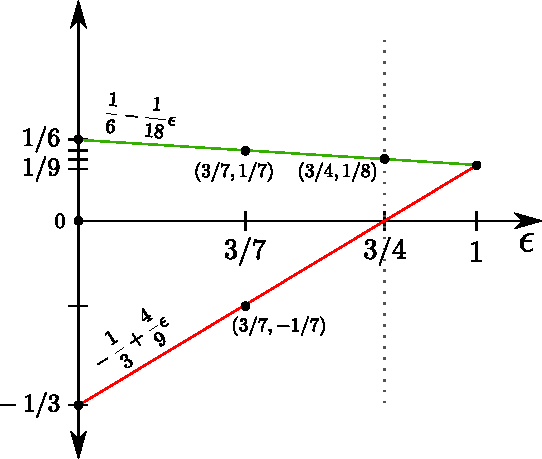
\includegraphics[scale=0.7]{figs/noisys.pdf}
    \caption{\textbf{Wigner components of the noisy Strange state.} 
    In the interval $0 \leq \epsilon < 3/7$, the negative component is larger than the positive components.
    At $\epsilon = 3/7$ the Wigner distribution is $(-\frac{1}{7},\frac{1}{7},\dots,\frac{1}{7})$.
    In the interval $3/7 < \epsilon < 3/4$, the positive components are larger than the negative component.
    In the interval $3/4 \leq \epsilon \leq 1$, there is no negativity.
    }
    \label{fig:noisys}
\end{figure}

The Wigner distribution of the $n$--copy $\epsilon$--noisy Strange state $\rho_{\rm{S}}(\epsilon)^{\otimes n}$ in the unital fragment is given by the convolution $\W{\rho_{\rm{S}}(\epsilon)^{\otimes n}} = \rm{W}_{\rho_{\rm{S}}(\epsilon)}^{\otimes n}$.
In general, $\rho_{\rm{S}}(\epsilon)^{\otimes n}$ contains $n + 1$ distinct components, labelled $0,\dots, n$.
We present the distinct Wigner components of $\rho_{\rm{S}}(\epsilon)^{\otimes n}$ along with their multiplicites in~\cref{tab:lcsu}.
Note that LHS (RHS) refers to elbow coordinates $i$ on the left of and including (right of) the maximum, precisely
\begin{align}
&\text{LHS: } 0 \leq i \leq \left\lfloor \frac{n}{2} \right\rfloor ; \\
&\text{RHS: } \left\lfloor \frac{n}{2} \right\rfloor +1 \leq i \leq n.
\end{align}
\begin{table}[h]
  \def\arraystretch{1.5}
  \centering
  \begin{tabular}{c|c|c|r|r}
    \multicolumn{3}{c|}{Case} & \multicolumn{1}{c}{$m_{i}(n, \epsilon)$} & \multicolumn{1}{|c}{$w_{i}(n, \epsilon)$} \\[0.5ex]\hline
    \multirow{4}{*}{\raisebox{-4ex}{\rotatebox[origin=c]{90}{$0\leq \epsilon < \frac{3}{7}$}}} & \hspace{0.8ex}\multirow{2}{*}{\raisebox{-1ex}{\rotatebox[origin=c]{90}{$n$ even}}}\hspace{0.8ex} & LHS & $8^{2i}\binom{n}{2i}$ & $\left( \frac{1}{6} - \frac{1}{18}\epsilon \right)^{2i}\left( -\frac{1}{3} + \frac{4}{9}\epsilon \right)^{n-2i}$ \\
    & & RHS & $8^{n-2i}\binom{n}{2i}$ & $\left( \frac{1}{6} - \frac{1}{18}\epsilon \right)^{n-2i}\left( -\frac{1}{3} + \frac{4}{9}\epsilon \right)^{2i}$ \\ \cline{2-5}
    & \multirow{2}{*}{\raisebox{-2ex}{\rotatebox[origin=c]{90}{$n$ odd}}} & LHS & $8^{2i+1}\binom{n}{2i+1}$ & $\left( \frac{1}{6} - \frac{1}{18}\epsilon \right)^{2i+1}\left( -\frac{1}{3} + \frac{4}{9}\epsilon \right)^{n-2i-1}$ \\
    & & RHS & $8^{n-2i-1}\binom{n}{2i+1}$ & $\left( \frac{1}{6} - \frac{1}{18}\epsilon \right)^{n-2i-1}\left( -\frac{1}{3} + \frac{4}{9}\epsilon \right)^{2i+1}$ \\ \hline
    \multirow{4}{*}{\raisebox{-4ex}{\rotatebox[origin=c]{90}{$\frac{3}{7}\leq \epsilon < \frac{3}{4}$}}} & \multirow{2}{*}{\raisebox{-1ex}{\rotatebox[origin=c]{90}{$n$ even}}} & LHS & $8^{n-2i}\binom{n}{2i}$ & $\left( \frac{1}{6} - \frac{1}{18}\epsilon \right)^{n-2i}\left( -\frac{1}{3} + \frac{4}{9}\epsilon \right)^{2i}$ \\
    & & RHS & $8^{2i}\binom{n}{2i}$ & $\left( \frac{1}{6} - \frac{1}{18}\epsilon \right)^{2i}\left( -\frac{1}{3} + \frac{4}{9}\epsilon \right)^{n-2i}$ \\ \cline{2-5}
    & \multirow{2}{*}{\raisebox{-2ex}{\rotatebox[origin=c]{90}{$n$ odd}}} & LHS & $8^{n-2i}\binom{n}{2i}$ & $\left( \frac{1}{6} - \frac{1}{18}\epsilon \right)^{n-2i}\left( -\frac{1}{3} + \frac{4}{9}\epsilon \right)^{2i}$ \\
    & & RHS & $8^{2i}\binom{n}{2i}$ & $\left( \frac{1}{6} - \frac{1}{18}\epsilon \right)^{2i}\left( -\frac{1}{3} + \frac{4}{9}\epsilon \right)^{n-2i}$ \\ \hline
  \end{tabular}
  \caption{Wigner components $w_{i}(n, \epsilon)$ of $\rho_{\rm{S}}(\epsilon)^{\otimes n}$ along with their multiplicities $m_{i}(n, \epsilon)$ in decreasing order in $i,\ 0 \leq i \leq n$.
  The order changes depending on the noise level $\epsilon$, the parity of the number of copies $n$ and the parity of the components (LHS vs RHS).
  Multiplication $2i$ is considered modulo $(n+1)$.}
  \label{tab:lcsu}
\end{table}

For example, the distribution of state $\rho_{\rm{S}}(0)^{\otimes 2}$ is
\begin{equation*}
	\begin{split}
	\rm{W}_{\rho_{\rm{S}}(0)^{\otimes 2}} = \Bigg( &\overbrace{\left( -\frac{1}{3} \right)^2}^1, \overbrace{\left( \frac{1}{6} \right)^2, \dots, \left( \frac{1}{6} \right)^2}^{64}, \\
	&\overbrace{ -\frac{1}{3} \cdot \frac{1}{6}, \dots, -\frac{1}{3} \cdot \frac{1}{6}}^{16} \Bigg)
	\end{split}
\end{equation*}

Every standard Lorenz curve contains $n$ elbows, labelled by 
\begin{equation*}
\{(x_{i}, L_{i})\}_{i=-1,0,\dots,n}\ ,
\end{equation*}
where the boundary points $(x_{-1}, L_{-1}) = (0,0)$ and $(x_{n}, L_{n}) = (1,1)$ are also included.
The maximum is the $(\lfloor n/2 \rfloor)$-th elbow and its coordinates are calculated by collecting all the positive Wigner components,
\begin{align}
	x_{\lfloor n/2 \rfloor} &= \frac{1}{2}\left(1 + \left(\frac{7}{9}\right)^n\right), \\
	L_{\lfloor n/2 \rfloor} &= \frac{1}{2}\left (1 + \left(\frac{15 - 8\epsilon}{9}\right)^n \right).
\end{align}
%\sum_{j: even}^n a^j \binom{n}{j} = \frac{1}{2} [ (1+a)^n + (1-a)^n ]

Expressions for all the elbow coordinates follow from summing up the Wigner components in decreasing order and we present the elbow coordinates for standard Lorenz curves in~\cref{tab:lcsu_coord_elb_app}.
\begin{table}[h]
  \def\arraystretch{1.5}
  \centering
  \begin{tabular}{c|c|c|r|r}
    \multicolumn{3}{c|}{Case} & \multicolumn{1}{c}{$x_{i}$} & \multicolumn{1}{|c}{$L_{i}$} \\[0.5ex]\hline
    \multirow{4}{*}{\raisebox{-5ex}{\rotatebox[origin=c]{90}{$0\leq \epsilon < \frac{3}{7}$}}} & \hspace{0.8ex}\multirow{2}{*}{\raisebox{-3ex}{\rotatebox[origin=c]{90}{$n$ even}}}\hspace{0.8ex} & LHS & $\Phi_+\left(2i;n,\frac{8}{9}\right)$ & $\left( \frac{5}{3} - \frac{8}{9}\epsilon\ \right)^n \Phi_+\left(2i;n,\frac{12-4\epsilon}{15-8\epsilon}\right)$ \\
    & & RHS & $x_{\lfloor n/2 \rfloor} + \Phi_-\left(2i;n,\frac{1}{9}\right)$ & $L_{\lfloor n/2 \rfloor} - \left( \frac{5}{3} - \frac{8}{9}\epsilon\ \right)^n\Phi_-\left(2i;n,\frac{3-4\epsilon}{15-8\epsilon}\right)$ \\ \cline{2-5}
    & \multirow{2}{*}{\raisebox{-3ex}{\rotatebox[origin=c]{90}{$n$ odd}}} & LHS & $\Phi_-\left(2i;n,\frac{8}{9}\right)$ & $\left( \frac{5}{3} - \frac{8}{9}\epsilon\ \right)^n \Phi_-\left(2i;n,\frac{12-4\epsilon}{15-8\epsilon}\right)$ \\
    & & RHS & $x_{\lfloor n/2 \rfloor} + \Phi_-\left(2i;n,\frac{1}{9}\right)$ & $L_{\lfloor n/2 \rfloor} - \left( \frac{5}{3} - \frac{8}{9}\epsilon\ \right)^n\Phi_-\left(2i;n,\frac{3-4\epsilon}{15-8\epsilon}\right)$ \\ \hline
    \multirow{4}{*}{\raisebox{-5ex}{\rotatebox[origin=c]{90}{$\frac{3}{7}\leq \epsilon < \frac{3}{4}$}}} & \multirow{2}{*}{\raisebox{-3ex}{\rotatebox[origin=c]{90}{$n$ even}}} & LHS & $\Phi_+\left(2i;n,\frac{1}{9}\right)$ & $\left( \frac{5}{3} - \frac{8}{9}\epsilon\ \right)^n \Phi_+\left(2i;n,\frac{3-4\epsilon}{15-8\epsilon}\right)$ \\
    & & RHS & $x_{\lfloor n/2 \rfloor} + \Phi_-\left(2i;n,\frac{8}{9}\right)$ & $L_{\lfloor n/2 \rfloor} - \left( \frac{5}{3} - \frac{8}{9}\epsilon\ \right)^n\Phi_-\left(2i;n,\frac{12-4\epsilon}{15-8\epsilon}\right)$ \\ \cline{2-5}
    & \multirow{2}{*}{\raisebox{-3ex}{\rotatebox[origin=c]{90}{$n$ odd}}} & LHS & $\Phi_+\left(2i;n,\frac{1}{9}\right)$ & $\left( \frac{5}{3} - \frac{8}{9}\epsilon\ \right)^n \Phi_+\left(2i;n,\frac{3-4\epsilon}{15-8\epsilon}\right)$ \\
    & & RHS & $x_{\lfloor n/2 \rfloor} + \Phi_+\left(2i;n,\frac{8}{9}\right)$ & $L_{\lfloor n/2 \rfloor} - \left( \frac{5}{3} - \frac{8}{9}\epsilon\ \right)^n\Phi_+\left(2i;n,\frac{12-4\epsilon}{15-8\epsilon}\right)$ \\ \hline
  \end{tabular}
  \caption{Standard Lorenz curves elbow coordinates.
  The expresion depends on the noise level $\epsilon$, the parity of the number of copies $n$ and the location of the elbow relative to the maximum (LHS vs RHS).
  Multiplication $2i$ is considered modulo $(n+1)$.
  Note that the Lorenz curve boundary points are $(x_{-1}, L_{-1}) \coloneqq (0,0)$ and $(x_{n}, L_{n}) = (1,1)$.
  }
  \label{tab:lcsu_coord_elb_app}
\end{table}

\subsection{Standard Lorenz curve coordinates}\label{app:lcsu_coord}
We can get explicit expressions for all $9^{n}$ points of the standard Lorenz curve $\lc{\rho_{\rm{S}}(\epsilon)^{\otimes n}}{\id/3}$, in terms of the elbow coordinates:
\begin{align}
    x_{ij} &= \left( 1-\frac{j}{m_{i}} \right) x_{i-1} + \frac{j}{m_{i}} x_{i}, \label{eq:x}\\
    L_{ij} &= \left( 1-\frac{j}{m_{i}} \right) L_{i-1} + \frac{j}{m_{i}} L_{i} \label{eq:l}
\end{align}
for $j = 1,\dots,m_{i}$ and $i=0,\dots,n$, where multiplicities $m_i = m_i(n, \epsilon)$ are given in~\cref{tab:lcsu}.

For visualisation purposes, we plot the Lorenz curve of state $\rho_{\rm{S}}(0)^{\otimes 2}$.
\begin{figure}[t]
    \centering
    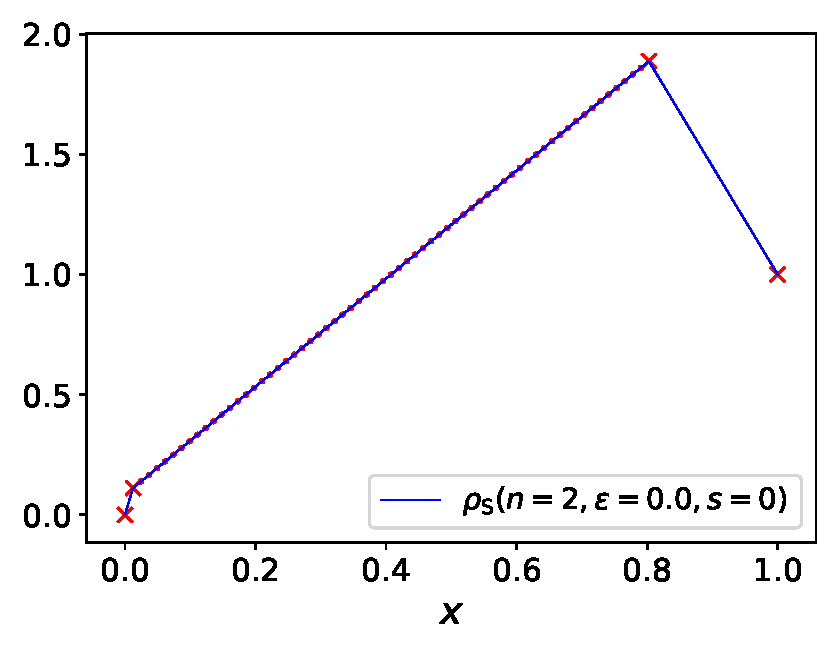
\includegraphics[scale=0.6]{figs/lcpoints.pdf}
    \caption{\textbf{All points on the Lorenz curve are uniformly distributed.}
    \cref{eq:x,eq:l}) capture the coordinates of all points up to the maximum.
    }
    \label{fig:lc}
\end{figure}

Consider the state 
\begin{equation*}
\rho_{\rm{S}}(n', \epsilon, n-n') \coloneqq \rho_{\rm{S}}(\epsilon)^{\otimes n'} \otimes \left( \frac{1}{3}\id \right)^{\otimes (n-n')},
\end{equation*}

Tensoring with the maximally mixed state keeps the Lorenz curve unchanged, but increases the resolution of (the uniformly distributed) points.
The new point coordinates are given by:
\begin{align}
    &x_{ijk} = \left( 1-p_{ijk}\right) x_{i-1} + p_{ijk} x_{i} \label{eq:lcsu_xcoord}\\
    &L_{ijk} = \left( 1-p_{ijk} \right) L_{i-1} + p_{ijk} L_{i}, \label{eq:lcsu_lcoord}\\
    &\text{where } p_{ijk} = \frac{k + (j-1)9^{n-n'}}{9^{n-n'} m_{i}} \nonumber\\
    &\text{for } i=0,\dots,n',\ j = 1,\dots,m_{i}(n', \epsilon') \text{ and } k = 1,\dots,9^{n-n'}. \nonumber
\end{align}

We can unify the indices, by introducing a single index
\begin{equation}
    I(i,j,k) \coloneqq k + \left[ (j-1) + \sum_{\ell=0}^{i-1} m_{\ell}(n', \epsilon') \right]9^{n-n'},
\end{equation}
so that $I=1,2,\dots, 9^{n}$.
The elbow coordinates correspond to 
\begin{equation}
	I(i, m_{i}(n', \epsilon'), 9^{n-n'}) = \sum_{\ell=0}^{i} m_{\ell}(n', \epsilon'),\ i= 0,\dots,n'.
\end{equation}
The index function $I$ is bijective, i.e.
\begin{equation}
	(i,j,k) = (i',j',k') \Leftrightarrow I(i,j,k) = I(i',j',k').
\end{equation}

\subsection{Strange state MSD in the unital fragment}\label{app:lc_compare}
Consider the Strange state MSD process in the unital fragment,
\begin{equation}\label{eq:su_conversion}
    \rho_{\rm{S}}(n', \epsilon, 0) \xrightarrow{\mathcal{O}_{\id/3}} \rho_{\rm{S}}(n', \epsilon', n-n').
\end{equation}
We denote initial state indices without a prime and target state indices with a prime,
\begin{align}
    I(i,j,k=1) &= j + \sum_{\ell=0}^{i-1} m_{\ell}(n, \epsilon), \\
    I'(i',j',k') &= k' + \left[ (j'-1) + \sum_{\ell=0}^{i'-1} m_{\ell}(n', \epsilon') \right]9^{n-n'}.
\end{align}

Pointwise Lorenz curve comparison requires $x_{I} = x_{I'}$, so the question is: 
\begin{center}
\emph{Given a triplet $(i',j',k')$, what is the tuple $(i,j)$ such that $I(i,j) = I'(i',j',k')$?}
\end{center}

According to~\cref{thm:elbows} which is proved in~\cref{app:lc_constraints}, for standard Lorenz curves, we need to match indices at the target state elbows, so the requirement on the indices is finding a tuple $(i, j)$, such that for a given $i' = 0,\dots,n'$,
\begin{equation}
	j + \sum_{\ell=0}^{i-1} m_{\ell}(n, \epsilon) = \sum_{\ell=0}^{i'} m_{\ell}(n', \epsilon').
\end{equation}

As a basic example, consider the process 
\begin{equation}
\rho_{\rm{S}}(\epsilon)^{\otimes 4} \xrightarrow{\mathcal{O}_{\id/3}} \rho_{\rm{S}}(\epsilon')^{\otimes 2} \otimes \left( \frac{1}{3}\id \right)^{\otimes 2}.
\end{equation}
We want to check which Lorenz curve is higher at the first elbows of the target state, i.e. we want to verify or reject the first inequality below:
\begin{equation}
	L_{I(i,j)} \geq L'_{I'(0, 1, 81)}
\end{equation}
where the first multiplicity of the target state is $m_0 = 1$.
The multiplicities of the initial state are $(1, 384, 4096)$.

The challenge is to find $i,j$ such that $i(i,j) = i'(0,1,81)$.
\nick{By trial and error}, we find that $(i,j) = (1, 80)$.
Now we can use~\cref{eq:lcsu_lcoord} to directly calculate
\begin{align*}
	L'_{i'(0,1,81)} &= L'_0 = \left( \frac{5}{3} - \frac{8}{9}\epsilon\ \right)^2 \Phi_+\left(0;2,4\frac{3-\epsilon}{15-8\epsilon}\right), \\
	L_{i(1, 80)} &= \left(1-\frac{80}{384} \right) L_0 + \frac{80}{384} L_1 \\
	\begin{split}
	&= \left( \frac{5}{3} - \frac{8}{9}\epsilon\ \right)^4 \bigg[ \frac{19}{24} \Phi_+\left(0;4,4\frac{3-\epsilon}{15-8\epsilon}\right) \\ 
	&\qquad + \frac{5}{24}\Phi_+\left(2;4,4\frac{3-\epsilon}{15-8\epsilon}\right) \bigg],
	\end{split}
\end{align*}
and then compare them.

%%%%%%%%%%%%%%%%%%%%%%%%%%%%%%%%%%%%%%%%

\section{Technical details of bound derivation in stabiliser fragments}
\label{app:lcst_technical}

\subsection{First and last elbow conditions}
\label{app:elb_constraints}
Here we prove the majorization constraints that arise by considering the first and last elbow of the initial stata only.
\begin{proposition}\label{prop:first_elb}
	Consider a magic state interconversion as in~\cref{eq:stdist}, where we denote by $(x_0, L_0)$ and $(x'_0, L'_0)$ the first elbow coordinates of the initial and target states respectively.
	If $x_0 < x'_0$, then it holds that
\begin{equation}\label{eq:first_elb_bound1}
	\frac{L_0}{x_0} \geq \frac{L_0'}{x_0'}.
\end{equation}
\end{proposition}
\begin{proof}
	Consider the Lorenz curve constraint at $x = x_0$,
\begin{equation}
	\lc{\rho}{\sigma}(x_0) \geq \lc{\tau}{\sigma}(x_0).
\end{equation}
Since $x_0 < x'_0$, we can find the target state Lorenz curve coordinate $L'_\star$ at location $x = x_0$ by interpolating between the origin and the target state's first elbow, 
\begin{equation}
	L'_\star = \frac{x_0}{x'_0}L'_0.
\end{equation}
We need $L_0 \geq L_\star'$ and rearranging we get~\cref{eq:first_elb_bound1}.
\end{proof}

\begin{proposition}\label{prop:last_elb}
	Consider a magic state interconversion as in~\cref{eq:stdist}, where we denote by $(x_E, L_E)$ and $(x'_E, L'_E)$ the last elbow coordinates of the initial and target states respectively.
	If $x_E > x'_E$, then it holds that
\begin{equation}\label{eq:last_elb_bound1}
	L_E \geq 1 + \frac{1-x_E}{1-x_E'} (L_E' - 1).
\end{equation}
\end{proposition}
\begin{proof}
	Consider the Lorenz curve constraint at $x = x_E$,
\begin{equation}
	\lc{\rho}{\sigma}(x_E) \geq \lc{\tau}{\sigma}(x_E).
\end{equation}
Since $x_E > x'_E$, we can find the target state Lorenz curve coordinate $L'_\star$ at location $x = x_E$ by interpolating between the the end-point $(1,1)$ and the target state's last elbow, 
\begin{equation}
	L'_\star = -\frac{L_E' - 1}{1 - x_E'}x_E + \frac{L_E' - x_E'}{1 - x_E'}.
\end{equation}
We need $L_E \geq L_\star'$ and rearranging we get~\cref{eq:last_elb_bound1}.
\end{proof}

\subsection{Component-multiplicity pairs}
\label{app:cmpairs}
In general, a $1$--copy $d$--dimensional state $\rho$ is defined exactly by its $d^2$--dimensional Wigner distribution $\W{\rho}$. 
The distribution $\W{\rho}$ is usually defined on the phase space, but it can be convenient to define it using pure vector notation. 
In particular, we introduce a component vector $\bmw(\rho) = (w_i)_{i=1,\dots,D}$ and a multiplicity vector $\bmm(\rho) = (m_i)_{i=1,\dots,D}$, where $D \leq d^2$ which together form a set of component-multiplicity pairs $\{(w_i, m_i)\}_{i=1,\dots,D}$.
\begin{definition}
	Consider a distribution $W$ and a positive integer $D \leq {\rm{dim}}\hspace{1pt}W$. 
	We call the set of ordered pairs $\{(w_i, m_i)\}_{i=1,\dots,D}$ a \emph{complete set of component-multiplicity pairs}, if $W$ contains $m_i$ components $w_i$ and $\sum_{i=0}^D m_i = d^2$.
\end{definition}
Therefore, such a set describes each component of $\W{\rho}$ exactly once.
As an example, two complete sets of pairs for the Strange state are $\{( -1/3, 1), ( 1/6, 8)\}$ and $\{(-1/3, 1), (1/6, 2), (1/6, 3), (1/6, 3)\}$.

Consider two states $\rho_A, \rho_B$ with Wigner distributions $\W{\rho_A}, \W{\rho_B}$ described respectively by complete sets of component-multiplicity pairs 
\begin{equation}
	\{(w_i, m_i)\}_{i=1,\dots,D_A} \text{ and } \{(w_j', m_j')\}_{j=0,\dots,D_B}.
\end{equation}
The multiplicative property of the Wigner distribution over a composite phase space $\cal{P}_{d_A} \times \cal{P}_{d_B}$ shown in~\cref{thm:wstate},
\begin{equation}
	\W[\bmx_A \oplus \bmx_B]{\rho_A \otimes \rho_B} = \W[\bmx_A]{\rho_A}\W[\bmx_B]{\rho_B},
\end{equation}
implies that the distribution $\W{\rho_A \otimes \rho_B}$ is $d_A^2 d_B^2$--dimensional and contains components of the form $w_i w_j'$. 
Therefore, the set $\{(w_i w_j', m_i m_j')\}$ with $i=1,\dots,D_A$ and $j=1,\dots,D_B$ is a complete set of component-multiplicity pairs for the distribution of the composite system $\W{\rho_A \otimes \rho_B}$.
This is true because all components are of the form $w_i w_j'$ and 
\begin{equation*}
	\sum_{i=1}^{D_A}\sum_{j=1}^{D_B} m_i m_j' = \sum_{i=1}^{D_A} m_i \sum_{j=1}^{D_B} m_j' = d_A^2 d_B^2.
\end{equation*}

Note that the rescaled distribution is also multiplicative,
\begin{align}
	&\widetilde{\rm{W}}_{\rho_A \otimes \rho_B | \gamma_A \otimes \gamma_B}(\bmx_A \oplus \bmx_B) = \frac{\W[\bmx_A \oplus \bmx_B]{\rho_A \otimes \rho_B}}{\W[\bmx_A \oplus \bmx_B]{\gamma_A \otimes \gamma_B}} = \nonumber \\
	&\frac{\W[\bmx_A]{\rho_A}\W[\bmx_B]{\rho_B}}{\W[\bmx_A]{\gamma_A}\W[\bmx_B]{\gamma_B}} = \widetilde{\rm{W}}_{\rho_A | \gamma_A}(\bmx_A)\widetilde{\rm{W}}_{\rho_B  | \gamma_B}(\bmx_B),
\end{align}
so a complete set of component-multiplicity pairs can be obtained for this distribution in the same fashion as for usual Wigner distributions.

Given a state $\rho$ and a complete set of component-multiplicity pairs describing its Wigner distribution $\W{\rho}$, we now provide a method of computing the components (and multiplicities) of the $n$--copy distribution $\W{\rho}^{\otimes n}$.
\begin{lemma}\label{lem:ncopycomponents}
	Let $W$ be a distribution defined by a complete set of component-multiplicity pairs $\{(w_i, m_i)\}_{i=1,\dots,D}$ with $D \leq {\rm{dim}}\hspace{1pt}W$ and consider the distribution $W^{\otimes n}$ obtained by taking the Kronecker product $W \otimes \dots \otimes W$ between $n$ copies of $W$.
	
	Denote by $C_D^n \coloneqq \{\bmk\}$ the set of all vectors $\bmk \coloneqq (k_1, \dots, k_D)$ with non-negative integer components that sum to $n$, i.e.
	\begin{equation*}
	0 \leq k_1, \dots, k_D \leq n \text{ and } k_1 + \dots + k_D = n.
	\end{equation*}
	
	Then, $W^{\otimes n}$ admits a complete set of component-multiplicity pairs $\{(W_{\bmk}, M_{\bmk})\}_{\bmk \in C_D^n}$, where
\begin{align}
	M_{\bmk} &= \frac{n!}{k_1!\dots k_D!} \prod\limits_{i=1}^D {m_i}^{k_i}, \label{eq:M}\\
	W_{\bmk} &= \prod\limits_{i=1}^D {w_i}^{k_i}. \label{eq:W}
\end{align}
\end{lemma}
\begin{proof}
	We proceed by induction.
	
	Assume $n = 1$.
	Let $\bmk_i$ be the vector with its $i$-th component equal to 1 and 0's elsewhere.
	The set $C_D^1$ consists of all vectors of this form, i.e. 
\begin{equation*}
	C_D^1 = \{ \bmk_i \}_{i=1,\dots,D}
\end{equation*}
	It is also true by direct calculation that
\begin{equation*}
	\left( W_{\bmk_i}, M_{\bmk_i} \right) = (w_i, m_i).
\end{equation*}
Therefore, $\{ (W_{\bmk}, M_{\bmk}) \}_{\bmk \in C_D^1}$ is a complete set of component-multiplicity pairs for $W$.

	Assume that $\{(W_{\bmk}, M_{\bmk})\}_{\bmk \in C_D^n}$ as given in~\cref{eq:M,eq:W} is a complete set of component-multiplicity pairs for the $n$--copy distribution $W^{\otimes n}$.
	By construction, the distribution $W^{\otimes (n+1)} = W^{\otimes n} \otimes W$ is multiplicative, so it admits the complete set of component multiplicity pairs
\begin{equation}
	\{(W_{\bmk} w_i, M_{\bmk} m_i)\},\ \bmk \in C_D^n \text{ and } i=1,\dots,D.
\end{equation}
	
	Consider the component sum of the distribution $W^{\otimes (n+1)}$,
\begin{align*}
	&\sum_{\bmk \in C_D^n}\sum_{i=1}^D M_{\bmk} m_i W_{\bmk} w_i = \sum_{\bmk \in C_D^n} M_{\bmk}W_{\bmk} \sum_{i=1}^D m_i w_i =\\
	&\sum_{\bmk \in C_D^n} \frac{n!}{k_1!\dots k_D!} \prod\limits_{i=1}^D {m_i}^{k_i}{w_i}^{k_i} \sum_{i=1}^D m_i w_i =\\
	&\left( \sum_{i=1}^D m_i w_i \right)^n \left( \sum_{i=1}^D m_i w_i \right) = \left( \sum_{i=1}^D m_i w_i \right)^{n+1} =\\
	&\sum_{\bmq \in C_D^{n+1}} M_{\bmq}W_{\bmq},
\end{align*}
where in the last expression, vectors $\bmq = (q_1, \dots, q_D)$ have non-negative integer components that sum to $(n+1)$ and 
\begin{align*}
	M_{\bmq} &= \frac{(n+1)!}{q_1!\dots q_D!} \prod\limits_{i=1}^D {m_i}^{q_i},\\
	W_{\bmq} &= \prod\limits_{i=1}^D {w_i}^{q_i}.
\end{align*}
We have used the multinomial theorem to proceed between lines 2-3 and lines 3-4 of the derivation.

We have achieved a regrouping of the distribution components.
Every component $W_{\bmq}$ is of the form $W_{\bmk} w_i$ with $q_i = k_i + 1$ and $q_j = k_j$ for $j\neq i$ and 
\begin{align*}
	\sum_{\bmq \in C_D^{n+1}}  \hspace{-6pt} M_{\bmq} =  \hspace{-10pt} \sum_{\bmq \in C_D^{n+1}} \frac{(n+1)!}{q_1!\dots q_D!} \prod\limits_{i=1}^D {m_i}^{q_i} = 
	\left( \sum_{i=1}^D m_i \right)^{n+1} \hspace{-10pt} = d^{n+1},
\end{align*}
which is the dimension of $W^{\otimes (n+1)}$.

Therefore, $\{ (W_{\bmq}, M_{\bmq}) \}_{\bmq \in C_D^{n+1}}$ is a complete set of component-multiplicity pairs for $W^{\otimes n}$, completing the proof.
\end{proof}

Index vector $\bmk$ has $D-1$ independent components and in the proof of our main theorem in~\cref{sec:stab} we have $D=4$, so we simplify the notation by writing the component and multiplicity vectors of the $n$--copy state distributions as $m_{ijk}, w(\rho_{\rm{S}})_{ijk}, w(\gamma)_{ijk}$ and $w(\rho_{\rm{S}}|\gamma)_{ijk}$, where $i,j,k$ are the 3 independent index components.

\subsection{First elbow location}
\label{app:first_elb_loc}
Consider a magic state interconversion in a stabilizer $\sigma$--fragment, as in~\cref{eq:stdist}, where we remind that $n \geq n'$ and we denote by $(x_0, L_0)$ and $(x'_0, L'_0)$ the first elbow coordinates of the initial and target states respectively.

Here, we show that $x_0 \leq x'_0$ for any of the three scenarios outlined in the proof of our main theorem in~\cref{sec:stab}.\\

1. $\rm{(C1)} \rightarrow \rm{(C1)}$.
We know from statistical physics that $e^{-\beta E_0} / \Z_\beta \leq 1$, so
	\begin{align*}
		x_0 &= \left(\dfrac{e^{-\beta E_0}}{3\Z_\beta}\right)^n = \left(\dfrac{e^{-\beta E_0}}{3\Z_\beta}\right)^{n-n'} \left(\dfrac{e^{-\beta E_0}}{3\Z_\beta}\right)^{n'} \\
		&< \left(\dfrac{e^{-\beta E_0}}{3\Z_\beta}\right)^{n'} = x_0'		
	\end{align*}

2. $\rm{(C2)} \rightarrow \rm{(C1)}$.
We now use the slightly altered inequality $e^{-\beta E_{\rm{max}}} / \Z_\beta \leq 1$ to proceed,
	\begin{align*}
		x_0 &= \left(\dfrac{e^{-\beta E_{\rm{max}}}}{\Z_\beta}\right)^n = \dfrac{e^{-\beta(n E_{\rm{max}} - n' E_0)}}{\Z_\beta^{n-n'}} \left(\dfrac{e^{-\beta E_0}}{3\Z_\beta}\right)^{n'} \\
		&\leq \dfrac{e^{-\beta(n E_{\rm{max}} - n' E_0)}}{e^{-\beta (n-n') E_{\rm{max}}}} \left(\dfrac{e^{-\beta E_0}}{3\Z_\beta}\right)^{n'} \\
		&= e^{-\beta n' (E_{\rm{max}} - E_0)} \left(\dfrac{e^{-\beta E_0}}{3\Z_\beta}\right)^{n'} \\
		&\leq \left(\dfrac{e^{-\beta E_0}}{3\Z_\beta}\right)^{n'} = x_0'.
	\end{align*}

3. $\rm{(C2)} \rightarrow \rm{(C2)}$.
Similarly in this scenario,
	\begin{align*}
		x_0 &= \left(\dfrac{e^{-\beta E_{\rm{max}}}}{\Z_\beta}\right)^n = \left(\dfrac{e^{-\beta E_{\rm{max}}}}{\Z_\beta}\right)^{n-n'} \left(\dfrac{e^{-\beta E_{\rm{max}}}}{\Z_\beta}\right)^{n'} \\
		&\leq \left(\dfrac{e^{-\beta E_{\rm{max}}}}{\Z_\beta}\right)^{n'} = x_0'	
	\end{align*}
	
	

\nick{LAST ELBOW BOUND}

To find the coordinates of the \textbf{last} elbow $(x_E, L_E)$, where $E$ is the number of elbows, we need to evaluate the minimum rescaled component,
\begin{align}
	&\bmw(\rho_{\rm{S}} | \sigma)_{\rm{min}} \coloneqq (3\Z)^{n}\times \nonumber\\
	&\min\limits_{i,j,k}\Big\{ (-v)^{n-\alpha} u^{\alpha} e^{\beta (n-\alpha)E_0} e^{\beta ( i E_0 + j E_1 + k E_2 )} \Big\}, \label{eq:min_slope}
\end{align}
where $0 \leq i,j,k \leq n$ and $\alpha \coloneqq i+j+k \leq n$.
Notice that for $0 \leq \epsilon \leq 3/7$, we have $v \geq u$. 
We need the sum $\alpha = i+j+k$ to be odd for the expression to be negative.

Given an odd value for the sum $\alpha$, the term $v^{n-\alpha} u^{\alpha} e^{-\beta (n-\alpha)E_0}$ is fixed (and negative), so the expression is minimised by setting the coefficient of the highest energy $E_{\rm{max}}$ equal to $\alpha$.
Hence, we have
\begin{align}
	&\bmw(\rho_{\rm{S}} | \sigma)_{\rm{min}} = \nonumber\\
	&-(3\Z)^{n} v^n e^{n\beta E_0}\max\limits_{\substack{\alpha = 1,3, \\ \dots,n-1}}{\Big\{ \left( \frac{u}{v} e^{\beta (E_{\rm{max}} - E_0)} \right)^{\alpha} \Big\}}.
\end{align}
If the expression $\frac{u}{v} e^{\beta (E_{\rm{max}} - E_0)}$ is less than $1$ then the minimum occurs at $\alpha=1$, otherwise it occurs at $\alpha = n-1$.

The minimum rescaled component can then be expressed as
\begin{equation}
\bmw(\rho_{\rm{S}} | \sigma)_{\rm{min}} =
	\begin{cases}
		-(3\Z)^{n} v^{n-1} u e^{\beta [(n-1)E_0 + E_{\rm{max}}]}, &\epsilon \leq \epsilon_{\star},\ \hspace{3pt}\rm{(C1)}	\\
		-(3\Z)^{n} v u^{n-1} e^{\beta [E_0 + (n-1)E_{\rm{max}}]}, &\epsilon > \epsilon_{\star}.\ \hspace{5pt}\rm{(C2)} 
	\end{cases}
\end{equation}
Case $\rm{(C1)}$ can correspond to $(i,j,k) = (1,0,0)$ if $E_{\rm{max}} = E_0$, when the multiplicity is $m_{100} = 2n$ and the corresponding Wigner components are $\bmw(\rho_{\rm{S}})_{100}, \bmw(\sigma)_{100}$ or it can correspond to $(i,j,k) = (0,1,0)$ ($(i,j,k) = (0,0,1)$), if $E_{\rm{max}} = E_1$ ($E_{\rm{max}} = E_2$), when the multiplicity is $m_{010} = 3n$ ($m_{001} = 3n$) and the corresponding Wigner components are $\bmw(\rho_{\rm{S}})_{010}, \bmw(\sigma)_{010}$ ($\bmw(\rho_{\rm{S}})_{001}, \bmw(\sigma)_{001}$).
Case $\rm{(C2)}$ corresponds to $(i,j,k) = (0,n-1,0)$ ($(i,j,k) = (0,0,n-1)$)
if we have $E_{\rm{max}} = E_1$ ($E_{\rm{max}} = E_2$), when the multiplicity is $m_{0,n-1,0} = 3^{n-1}n$ ($m_{0,0,n-1} = 3^{n-1}n$) and the corresponding Wigner components are $\bmw(\rho_{\rm{S}})_{0,n-1,0}, \bmw(\sigma)_{0,n-1,0}$ ($\bmw(\rho_{\rm{S}})_{0,0,n-1}, \bmw(\sigma)_{0,0,n-1}$).

The last elbow coordinates can finally be derived by sutracting the appropriate rescaled component from 1, $(x_E, L_E) =$
\begin{equation}\label{eq:last_elb_coords}
	\begin{cases}
		&\left( 1-\dfrac{2n}{(3\Z_\beta)^n}e^{-\beta [(n-1)E_0 + E_{\rm{max}}]},\ 1 + 2n v^{n-1} u \right), \vspace{5pt}\\
		&\hspace{5pt} \text{if } E_{\rm{max}} = E_0, \hspace{51pt}\rm{(C1a)} \vspace{10pt}\\
		&\left( 1-\dfrac{3n}{(3\Z_\beta)^n}e^{-\beta [(n-1)E_0 + E_{\rm{max}}]},\ 1 + 3n v^{n-1} u \right), \vspace{5pt}\\
		&\hspace{5pt} \text{if } E_{\rm{max}} > E_0, \epsilon \leq \epsilon_{\star}, \hspace{20pt}\rm{(C1b)} \vspace{10pt}\\
		&\left( 1-\dfrac{n}{3\Z_\beta^n}e^{-\beta [E_0 + (n-1)E_{\rm{max}}]},\ 1 + 3^{n-1}n v u^{n-1} \right), \vspace{5pt}\\
		&\hspace{5pt} \text{if } E_{\rm{max}} > E_0, \epsilon \geq \epsilon_{\star}. \hspace{22pt}\rm{(C2)}
	\end{cases}
\end{equation}

Assuming that $E_{\rm{max}} > E_0$ for clarity, we have the same three scenarios as in the case of the first elbow bound:
\begin{enumerate}
	\item $\rm{(C1)} \rightarrow \rm{(C1)}$ if $\beta < \beta_{\star}$ and $\epsilon' < \epsilon  \leq \epsilon_{\star}$.
	\item $\rm{(C2)} \rightarrow \rm{(C1)}$ if $\beta < \beta_{\star}$ and $\epsilon' \leq \epsilon_{\star} < \epsilon$.
	\item $\rm{(C2)} \rightarrow \rm{(C2)}$ if $\beta < \beta_{\star}$ and $\epsilon_{\star} \leq \epsilon' < \epsilon$ or $\beta \geq \beta_{\star}$.
\end{enumerate}
Now the last elbow condition on Lorenz curves can be derived by simple interpolation, giving the condition
\begin{equation}
	L_E \geq 1 + \frac{1-x_E}{1-x_E'} (L_E' - 1),
\end{equation}
provided that the last elbow location is closer to 1 for the initial state than the target state, which is always true.

The last elbow bound then can be rephrased in terms of the first elbow bound as $R_{\rm{last-elb}} - R_{\rm{first-elb}} = $
\begin{equation}\label{eq:last_elb_coords}
	\begin{cases}
		\dfrac{1}{n} \dfrac{\log{\frac{u(\epsilon)v(\epsilon')}{u(\epsilon')v(\epsilon)}}}{\ln{\big( 1-\frac{4}{3}\epsilon' \big)} + \beta (E_0 - F(\beta))},\ &\rm{(C1)} \rightarrow \rm{(C1)}, \vspace{10pt}\\
		\dfrac{1}{n} \dfrac{\log{\frac{v(\epsilon)v(\epsilon')}{u(\epsilon)u(\epsilon')}} - 2\beta(E_{\rm{max}} - E_0)}{\ln{\big( 1-\frac{4}{3}\epsilon' \big)} + \beta (E_0 - F(\beta))},\ &\rm{(C2)} \rightarrow \rm{(C1)}, \vspace{10pt}\\
		\dfrac{1}{n} \dfrac{\log{\frac{v(\epsilon')u(\epsilon')}{v(\epsilon')u(\epsilon)}}}{\ln{\big( \frac{1}{2}-\frac{1}{6}\epsilon' \big)} + \beta (E_{\rm{max}} - F(\beta))},\ &\rm{(C2)} \rightarrow \rm{(C2)}, 
	\end{cases}
\end{equation}

Note that the last elbow bounds have a dependence on $n$, which interestingly is due to $n$ being even.
Had we considered \textbf{odd} number of copies $n$, then the first elbow bound would depend on $n$ and the last elbow bound would not.
This, along with the unital fragment analysis, makes me think that calculating the bounds again for odd $n$ or $\epsilon > 3/7$ would reveal nice symmetries of the analysis, but it's probably not worth the time, so including last elbow analysis properly feels incomplete.

Determining the sign of the difference between the last and first elbow bounds tells us which bound is better.
The term $\log{\frac{u(\epsilon)v(\epsilon')}{u(\epsilon')v(\epsilon)}}$ is always positive for $\epsilon > \epsilon'$, therefore the last elbow bound, compared to the first elbow bound, is always \textbf{worse} in the first scenario and always \textbf{better} in the third scenario (remember, this is the yellow-ish right part of~\cref{fig:rate_contour}).

In the second scenario ($\rm{(C2)} \rightarrow \rm{(C1)}$), the expression looks very weird to me, seems like the difference tends to $-\infty$ as $E_{\rm{max}} \rightarrow \infty$.
I am a bit stuck with this expression and I am not sure it's worth putting more time in it.

%%%%%%%%%%%%%%%%%%%%%%%%%%%%%%%%%%%%%%%%



























